% I use a custom document class that can be found at
% github.com/mwhittaker/texmf. Honestly, it's a big pain in the butt to set it
% up. Sorry this document isn't easier to compile! If you have the hw document
% class set up, you can compile this document with `latexmk -pdf answers.tex`

\documentclass{hw}
\title{CS 5220 -- 2015-09-01 Preclass Questions}

\hypersetup{
  colorlinks = true,
  allcolors = blue,
}

\newcommand{\lasthw}{https://github.com/mwhittaker/lecture/blob/2015-08-27/2015-08-27/answers.pdf}

\begin{document}
\maketitle{}

\begin{enumerate}
  \item
    See \href{\lasthw{}}{here}.

  \item
    See \href{\lasthw{}}{here}.

  \item
    We have $t$ tasks and $p$ stages. Assume each task takes $k$ seconds. In
    the serial case, we require $tk$ seconds. In the parallel case, we wait $k$
    seconds for the first task to finish and then wait $\frac{k}{p}$ seconds
    for each of the next $(t - 1)$ tasks for a total of $k + (t -
    1)\frac{k}{p}$ seconds. This leads to a total speedup up $\frac{kt}{k +
    (t-1)\frac{k}{p}}$. If we let the number of tasks tend to infinity, we get
    \[
      \lim_{t \to \infty} \group{\frac{kt}{k + (t-1)\frac{k}{p}}} = p
    \]

  \item
    Serially, we require $1 + 0.5 + 0.25 + 0.5 + 0.5 = 2.75$ seconds. With an
    arbitrary number of processors, we can compile everything in $2.25$ seconds
    by compiling OpenMPI and OpenBLAS in parallel.

  \item
    Refer to \figref{localtimingsline} and \figref{localtimingsheat}.

  \item
    Refer to \figref{totienttimingsline} and \figref{totienttimingsheat}.

  \item
    An implementation of the centroid algorithms can be found in
    \texttt{centroid.c}. Algorithm a, b, and c take roughly 70, 130, and 120
    milliseconds to process 50,000,000 coordinates. I ran the code on my local
    computer, not on the cluster.

    To build and run the code, run \texttt{make \&\& ./centroid}. It will print
    the time taken by algorithm a, b, and c in milliseconds followed by the
    centroids computed by algorithms a, b, and c.
\end{enumerate}

\begin{figure}[h]
  \centering
  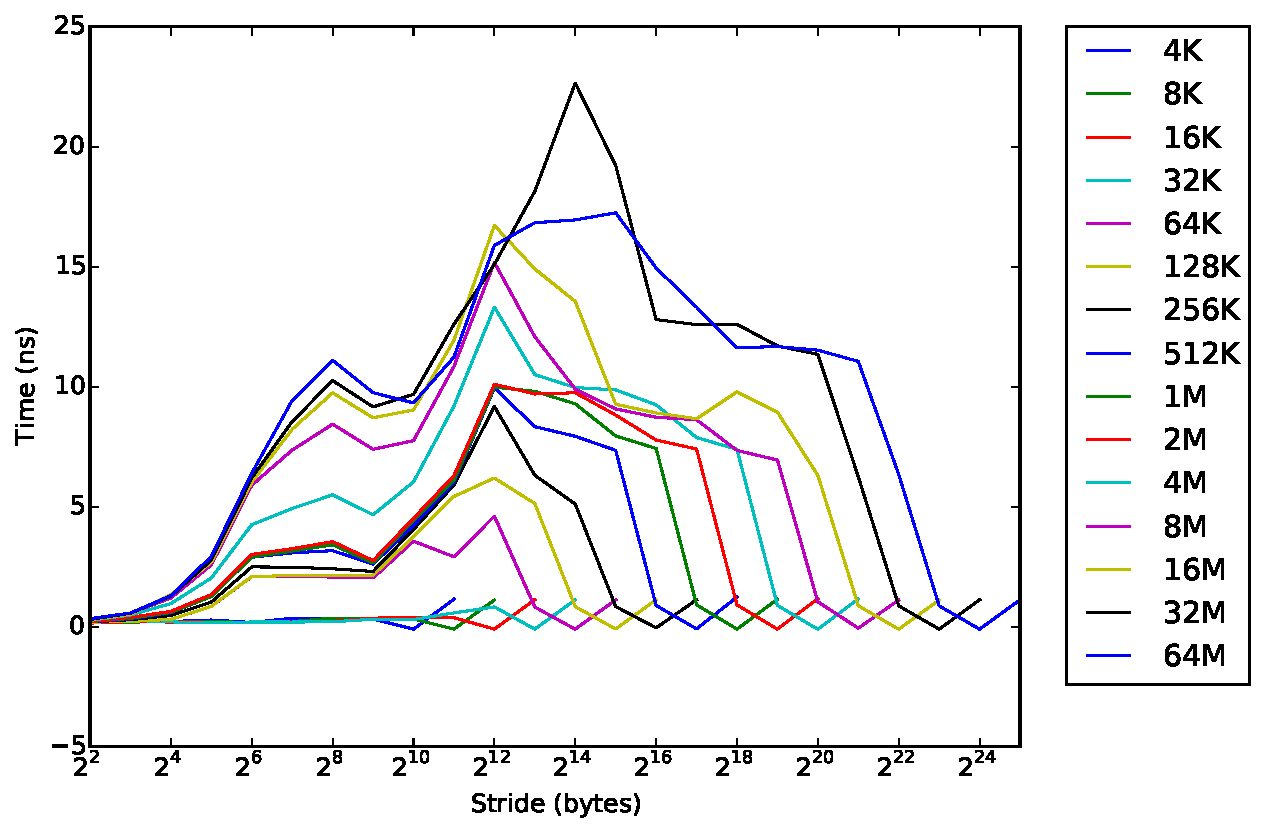
\includegraphics[width=0.9\textwidth]{timings-line.pdf}
  \caption{Local membench line plot.}
  \label{fig:localtimingsline}
\end{figure}

\begin{figure}[h]
  \centering
  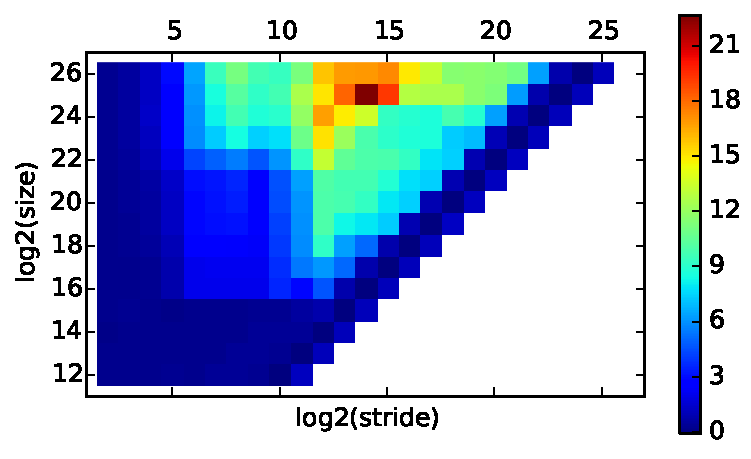
\includegraphics[width=0.9\textwidth]{timings-heat.pdf}
  \caption{Local membench heat plot.}
  \label{fig:localtimingsheat}
\end{figure}

\begin{figure}[h]
  \centering
  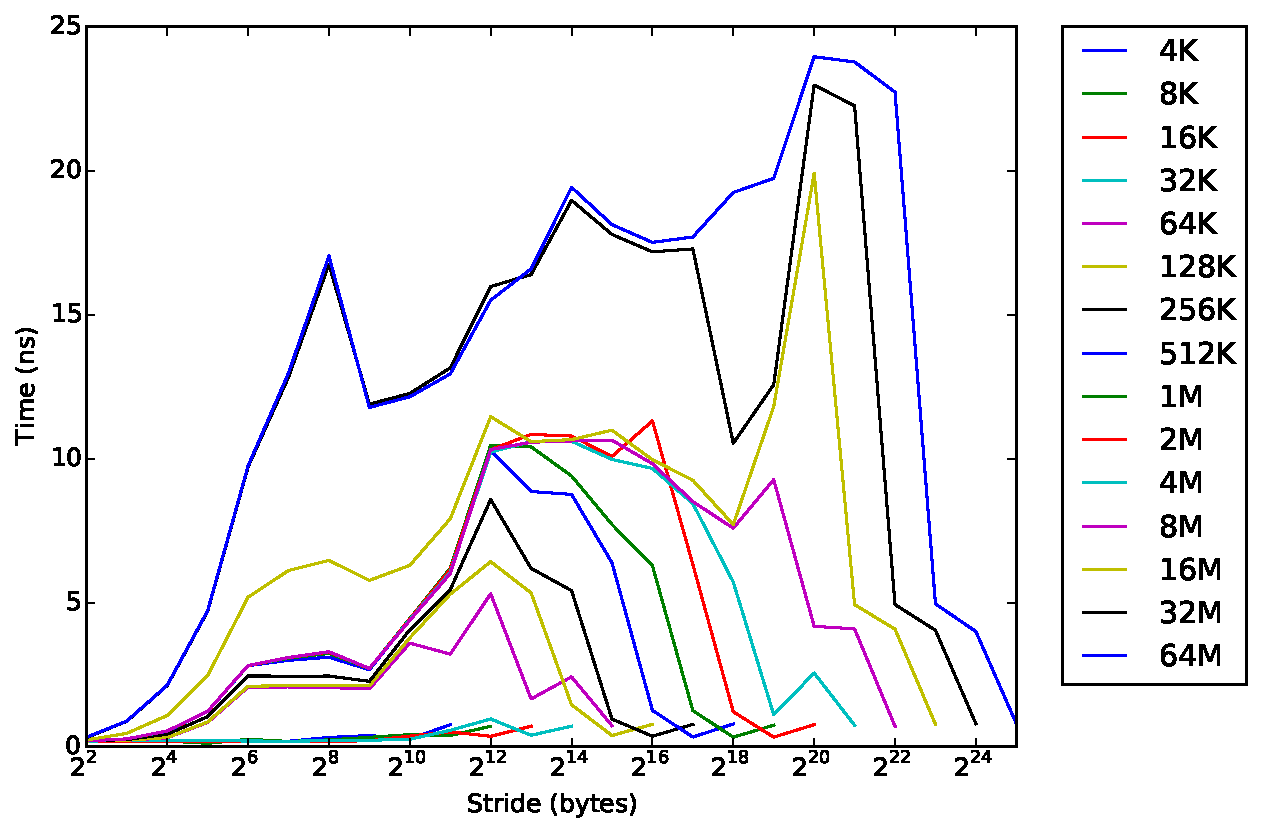
\includegraphics[width=0.9\textwidth]{timings-line-totient.pdf}
  \caption{Totient membench line plot.}
  \label{fig:totienttimingsline}
\end{figure}

\begin{figure}[h]
  \centering
  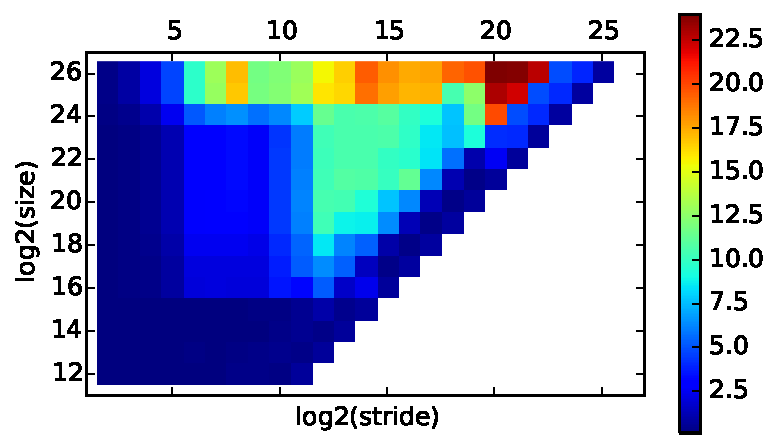
\includegraphics[width=0.9\textwidth]{timings-heat-totient.pdf}
  \caption{Totient membench heat plot.}
  \label{fig:totienttimingsheat}
\end{figure}
\end{document}
